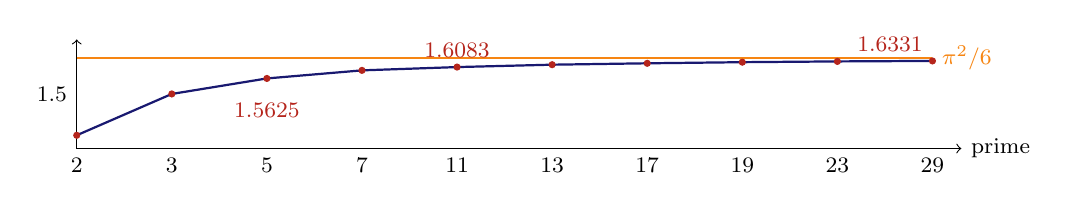
\begin{tikzpicture}[every node/.style={font=\footnotesize},x=1.05cm,y=3.15cm]
  \draw[->,black] (0,1.28)--(10.7,1.28) node[right] {prime};
  \draw[->,black] (0,1.28)--(0,1.72);
  \draw[BurntOrange,thick] (0,1.64493)--(10.35,1.64493);
  \node[BurntOrange,right] at (10.35,1.64493) {$\pi^2/6$};
  \draw[MidnightBlue,thick]
    (0,1.33333)--(1.15,1.50000)--(2.30,1.56250)--(3.45,1.59505)--(4.60,1.60834)
    --(5.75,1.61792)--(6.90,1.62354)--(8.05,1.62805)--(9.20,1.63113)--(10.35,1.63307);
  \foreach \x/\y in {0/1.33333,1.15/1.50000,2.30/1.56250,3.45/1.59505,4.60/1.60834,5.75/1.61792,6.90/1.62354,8.05/1.62805,9.20/1.63113,10.35/1.63307}
    \fill[BrickRed] (\x,\y) circle (1.3pt);
  \node[below] at (0,1.28) {$2$};
  \node[below] at (1.15,1.28) {$3$};
  \node[below] at (2.30,1.28) {$5$};
  \node[below] at (3.45,1.28) {$7$};
  \node[below] at (4.60,1.28) {$11$};
  \node[below] at (5.75,1.28) {$13$};
  \node[below] at (6.90,1.28) {$17$};
  \node[below] at (8.05,1.28) {$19$};
  \node[below] at (9.20,1.28) {$23$};
  \node[below] at (10.35,1.28) {$29$};
  \node[BrickRed,below] at (2.30,1.50) {$1.5625$};
  \node[BrickRed,above] at (4.60,1.60834) {$1.6083$};
  \node[BrickRed,above left] at (10.35,1.63307) {$1.6331$};
  \node[left] at (0,1.50) {$1.5$};
\end{tikzpicture}
